%INTENTO 1

%En el Capítulo \ref{cap:int} se detalló que el sisetma desarrollado se compone de tres componentes principales, a saber: El Host, cuyo rol es llevado a cabo por una PC; la interfaz, integrada por el controlador FX2LP de Cypress y un FPGA, en este caso un Spartan-6 de Xilinx. A su vez, el Capítulo \ref{cap:fpga}, indica que el sistema interno del FPGA lleva una Maquina de Estados Finitos (MEF), cuya función es la de realizar el efectivo intercambio de datos con la interfaz, y un sistema genérico.
%
%Hasta acá se ha desarrollado la configuración de la interfaz y la implementación de la MEF. Sin embargo, es necesario, que el sistema pueda funcionar en forma autónoma, proveerle un sistema mínimo que pueda hacer las veces de fuente y sumidero de datos. Es por esto, que se dotó al sistema con una memoria FIFO con el objetivo de implementar un eco que permita realizar una evaluación de desempeño de la comunicación desarrollada. Así, se permite enviar mensajes desde una PC y que estos sean recibidos luego.
%
%\subsection{Implementación de la memoria FIFO en el FPGA}
%	La memoria FIFO sintetizada en el FPGA se obtuvo a través de la herramienta {\it Core Generator} provista por Xilinx junto con el entorno de desarrollo ISE, utilizado en este trabajo para el desarrollo~\cite{XilinxInc}. La configruación seleccionada generó una memoria FIFO de 511 bytes, con puertos de entrada y salida dedicados, es decir uno de entrada y uno de salida, un bus de 16 bits de ancho. Posee señal de reconocimiento de escritura. También se dotó a la memoria generada con entradas de reloj y habilitación de bus independientes tanto para el puerto de entrada como el puerto de salida.
%	
%	
%INTENTO 2
%TODO debería decir como generar cada una de las señales internas propuesas en el capitulo correspondiente... la magen en cuestion es \ref{fpga:intersignal}
%Con el objetivo de verificar el sistema desarrollado, se procedió a implementarlo en un sistema mínimo que sea capaz de utilizar la comunicación, de forma tal que el Host pueda establecer un enlace con el FPGA. Para ello, se implementó un sistema eco, es decir, un sistema que recibe los mensajes que envía el Host y, luego, los transmite para que el Host pueda recibirlos. De esta forma, el Host puede reconocer que los datos enviados no fueron perdidos ni modificados.

% INTENTO 3
%El sistema desarrollado en el FPGA para realizar las pruebas de desempeño implementa la MEF desarrollada en el Capítulo \ref{cap:fpga}, debido a que es uno de los componentes principales en lo que a las pruebas se refieren. Sin embargo, el sistema también requiere de capacidad de almacenamiento de los datos que son provistos desde la PC y de una señal de reloj.

% INTENTO 4
Para realizar las pruebas de desempeño, se elaboró un sistema tipo Eco, es decir, un dispositivo que ante la recepción de un mensaje, responde con la retransmisión del mismo hacia el emisor original. En este caso, el emisor es la PC y el dispositivo que reenvía el mensaje es el FPGA. Para poder retransmitir el mensaje, se implementó el sistema presentado en el esquema de la Figura~\ref{test:fpga}. En ella se observa que el FPGA Spartan 6 fue dotado de un bloque con la MEF presentada en el Capítulo anterior. A dicho bloque, fue conectada una memoria FIFO. Así, los datos que son enviados desde la PC, se almacenan en la memoria FIFO a medida que arriban, atravesando la interfaz. Luego, estos datos son reenviados desde la misma memoria FIFO, emprendiendo el circuito hacia la PC.

La señal de reloj del FPGA Spartan 6 es provista por una de las salidas de un módulo PLL que el FPGA tiene incorporado. A tráves de este módulo, se disminuye la frecuencia de \SI{50}{\mega\hertz} que entrega el oscilador de la placa de desarrollo Mojo v3 a los \SI{48}{\mega\hertz} necesarios para el conectarse con el controlador FX2LP. La señal de reloj emitida por la salida del PLL sincroniza a todo el sistema implementado en el FPGA. 

Dos de los módulos implementados en el sistema de pruebas no fueron desarrollados en el presente trabajo, sino que se generaron a través de soluciones que provee la empresa Xilinx Inc. para el desarrollo de sistemas. Tanto el PLL como la memoria FIFO incorporadas al sistema implementado dentro del FPGA, fueron generadas por la herramienta \textit{Core Generator}, provista por la empresa Xilinx Inc. en el software de programación ISE. Las señales SLRD y SLWR debieron ser adaptadas para compatibilizar el funcionamiento de la memoria generada por la herramienta \textit{Core Generator}.

\begin{figure}[t]
	\centering
	\begin{tikzpicture}[scale=.7]
		\begin{scope}[transform shape,node distance=4,>=latex,double distance=1.3]
			\node[simple](mea)[]{Máquina de Estados Finitos};
			
			\node[simple,rounded corners](fx2lp)[left=of mea]{Interfaz USB};
			\draw[<->,double]([yshift=10*220/11]fx2lp.south east) --node[above]{FD[15:0]}([yshift=220/11*10]mea.south west);
			\draw[<-,double]([yshift=220/11*9]fx2lp.south east) --node[above]{FADDR[1:0]}([yshift=220/11*9]mea.south west);
			\draw[->]([yshift=220/11*8]fx2lp.south east) --node[above]{FLAGA}([yshift=220/11*8]mea.south west);
			\draw[->]([yshift=220/11*7]fx2lp.south east) --node[above]{FLAGB}([yshift=220/11*7]mea.south west);
			\draw[->]([yshift=220/11*6]fx2lp.south east) --node[above]{FLAGC}([yshift=220/11*6]mea.south west);
			\draw[->]([yshift=220/11*5]fx2lp.south east) --node[above]{FLAGD}([yshift=220/11*5]mea.south west);
			\draw[->]([yshift=220/11*4]fx2lp.south east) --node[above]{SLWR}([yshift=220/11*4]mea.south west);
			\draw[->]([yshift=220/11*3]fx2lp.south east) --node[above]{SLRD}([yshift=220/11*3]mea.south west);
			\draw[->]([yshift=220/11*2]fx2lp.south east) --node[above]{SLOE}([yshift=220/11*2]mea.south west);
			\draw[->]([yshift=220/11*1]fx2lp.south east) --node[above]{PKTEND}([yshift=220/11*1]mea.south west);
			
			
			\node[simple,minimum height=150,minimum width=50](interno)[right=6 of mea.north east,anchor=north west]{Memoria FIFO};
			\draw[double,->]([yshift=-1*150/8]mea.north east)--node[above]{Dato\_enviado[15:0]} ([yshift=-1*150/8]interno.north west);
			\draw[double,<-]([yshift=-2*150/8]mea.north east)--node[above]{Dato\_a\_enviar[15:0]}([yshift=-2*150/8]interno.north west);
			\draw[<-]([yshift=-3*150/8]mea.north east)--node[above]{Enviar\_datos}([yshift=-3*150/8]interno.north west);
			\draw[<-]([yshift=-4*150/8]mea.north east)--node[above]{PKTEND}([yshift=-4*150/8]interno.north west);
			
			\node[simple,minimum height=70](adapt)[anchor=south] at  ($(mea.south|-interno.south)!0.5!(interno.south)$|-interno.south) {Adaptador};
			\draw[->]([yshift=-5.5*150/6]mea.north east)--node[above]{SLWR}([yshift=-5.5*150/6]mea.north east -| adapt.west);
			\draw[->]([yshift=-4.5*150/6]mea.north east)--node[above]{SLRD}([yshift=-4.5*150/6]mea.north east -| adapt.west);
			\draw[<-]([yshift=1*70/5]adapt.south east) --node[above]{Llena} ([yshift=1*70/5]adapt.south east -| interno.west);
			\draw[<-]([yshift=2*70/5]adapt.south east) --node[above]{Vacia} ([yshift=2*70/5]adapt.south east -| interno.west);
			\draw[->]([yshift=3*70/5]adapt.south east) --node[above]{wr\_en} ([yshift=3*70/5]adapt.south east -|interno.west);
			\draw[->]([yshift=4*70/5]adapt.south east) --node[above]{rd\_en} ([yshift=4*70/5]adapt.south east -|interno.west);
			
			\node[simple,minimum size=50](clk) [anchor=south]at (mea.south west-|interno.south)  {PLL};
			\draw[<-]([yshift=15]mea.east |- clk.west)--node[above,near end]{Reloj}([yshift=15]clk.west);
			\draw[->] (clk) -- node[right]{clk} (interno);
			\draw[->] ([yshift=15]clk.west) -| (adapt);
			
			\node[rounded corners,simple, minimum size=50](clkSrc)[right=1 of clk]{Fuente de reloj};
			\draw[->](clkSrc) to (clk);
			
			\node[simple,minimum size=30](rst)[anchor=south]at($(mea.south)!.5!(clk.south)$) {Reset};
			\draw[->]([yshift=15]clk.west)-|(rst.north);
			\node[simple,rounded corners,minimum size=50](puls)[below=1 of rst]{Pulsador};
			\draw[->](rst.west) --node[above]{Reset} (rst.west -| mea.east);
			\draw[<-](rst.south)--(puls.north);
			
		\end{scope}
		\begin{scope}[]
			\node[rounded corners,inner ysep=5pt,draw=black,rectangle,fit={(clk)(mea)(interno)},label=north:FPGA](fpga){};
			\node[inner ysep=11pt, yshift= 8pt, draw=black,rectangle,fit={(puls)(fpga)(clkSrc)},label=north:Mojo](){};
		\end{scope}
	\end{tikzpicture}
	\caption{Diagrama en bloques del sistema implementado en el FPGA}
	\label{test:fpga}
\end{figure}

%La arquitectura del sistema implementado en la placa de desarrollo Mojo v3 se observa en el diagrama en bloques de la Figura \ref{test:fpga}. Los datos que provienen desde el controlador FX2LP (originados en la PC en forma previa), llegan al FPGA a través de la MEF. Luego, la MEF remite los datos arribados a la memoria FIFO.

%Las señales SLRD y SLWR debieron ser adaptadas para compatibilizar el funcionamiento de la memoria generada por la herramienta \textit{Core Generator}.

%La señal de reloj emitida por la salida del sincroniza tanto a la MEF como a la memoria FIFO. 

Por su parte, la placa Mojo v3 incorpora un pulsador, que es usado en este trabajo como señal de reset asíncrona. El sistema tiene un reset síncrono realizado a través de un contador, que es utilizado para establecer los valores iniciales del circuito.


%Para establecer un sistema eco, se deben implementar todas las señales de control que se observan en la Figura \ref{fpga:intersignal}. Estas son, señal de reset, señal de reloj, solicitud  sde envío de datos y los datos a enviar. A su vez, se deben poder leer los datos recibidos y las señales {\it SLWR} y {\it SLRD}, a través de las cuales el sistema señala el cambio de dato. 
%
%Con el objetivo de poder recibir, almacear y reenviar los datos que llegan desde la interfaz, se sintetizó en el FPGA una memoria FIFO que almacene los datos y, cuando el EP de salida no posee más datos, es decir que el {\it Flag Vacío} se encuentra activo, retransmita los datos hacia la interfaz hasta que el Host los solicite.
%
%Una vez incorporados los componentes al FPGA, se realizó su validación funcional antes de ser cargado todo el desarrollo al FPGA para efectuar las pruebas del sistema. A continuación, se detallarán los componentes y señales que se sintetizaron, como así también la verificación realizada.

%\subsection{Declaración de la entidad}
%	Para la implementación y síntesis del sistema, es necesario declarar los puertos que tendrán una correspondencia física con un pin de salida del FPGA en la descripción de mayor jerarquía. El archivo que posee una mayor jerarquía es usualmente llamada top.
%	
%	Como se conoce cuáles son las señales a través de las cuales el FPGA debe conectarse con la interfaz, es posible declarar la entidad que se sintetizó. Además se declararó  la señal de reloj, que proviene desde la placa Mojo v3. El código de descripción en donde se declaró la entidad se muestra a continuación.
%	
%	\begin{lstlisting}[language=VHDL,backgroundcolor=\color{gray!30}]
%entity fx2lp_interface_top is
%	generic(
%		constant in_ep_addr:	std_logic_vector(1 downto 0) := "00";
%		constant out_ep_addr:	std_logic_vector(1 downto 0) := "11";
%		constant port_width: integer := 16
%		);
%	port(
%		fdata   : inout std_logic_vector(port_width-1 downto 0);  
%		faddr   : out   std_logic_vector(1 downto 0);
%		slrd    : out   std_logic;
%		slwr    : out   std_logic;
%		flaga   : in    std_logic;
%		flagb   : in    std_logic;
%		flagc   : in    std_logic;
%		flagd   : in    std_logic;
%		sloe    : out   std_logic;
%		pktend  : out   std_logic;
%		clk_in  : in    std_logic
%		);
%end fx2lp_interface_top;
%	\end{lstlisting}
%
%\subsection{Instanciación de la MEF}
%		Dentro de los componentes incorporado al sistema, el más importante es la MEF elaborada en el Capitulo \ref{cap:fpga}, debido a que es el componente que se desea sintetizar, verificar y probar. Para que el sistema reconozca que ese módulo debe incorporarlo al sistema, se declaró como componente los puertos de la entidad elaborada en el capítulo mencionado y se lo instanció como se observa a continuación.
%		
%		\begin{lstlisting}[language=VHDL,backgroundcolor=\color{gray!30}]
% architecture fx2lp_interface_arq of fx2lp_interface_top is
% 	COMPONENT fx2lp_interface
%	GENERIC(
%		constant in_ep_addr:	std_logic_vector(1 downto 0) := "00";
%		constant out_ep_addr:std_logic_vector(1 downto 0) := "11";
%		constant port_width: integer := 16
%	);
%	PORT(
%		clk : IN std_logic;
%		reset : IN std_logic;
%		flaga : IN std_logic;
%		flagb : IN std_logic;
%		flagc : IN std_logic;
%		flagd : IN std_logic;
%		send_req : IN std_logic;
%		data_to_tx : IN std_logic_vector(15 downto 0);    
%		fdata : INOUT std_logic_vector(15 downto 0);      
%		faddr : OUT std_logic_vector(1 downto 0);
%		slrd : OUT std_logic;
%		slwr : OUT std_logic;
%		sloe : OUT std_logic;
%		pktend : OUT std_logic;
%		rx_data : OUT std_logic_vector(15 downto 0)
%		);
%	END COMPONENT;
% begin
% 	interface: fx2lp_interface PORT MAP(
%		clk => sys_clk,
%		reset => reset,
%		fdata => fdata,
%		faddr => faddr,
%		slrd => slrd_sig,
%		slwr => slwr_sig,
%		flaga => flaga,
%		flagb => flagb,
%		flagc => flagc,
%		flagd => flagd,
%		sloe => sloe,
%		pktend => pktend,
%		send_req => write_req,
%		rx_data => din,
%		data_to_tx => dout
%	);
%[...]
%end fx2lp_interface_arq;
%		\end{lstlisting}
%		
%		Se puede observar que las constantes genéricas fueron definidas en la declaración del componente . Sin embargo, estas no fueron instanciadas debido a que la configuración a probar era la asignada por defecto.
%
%\subsection{Implementación de sistemas adicionales}
%Dos de los módulos implementados en el sistema de pruebas no fueron desarrollados en el presente trabajo, sino que se generaron a través de soluciones que provee la empresa Xilinx Inc. para el desarrollo de sistemas.
%
%Los módulos provistos por Xilinx Inc. fueron el PLL, a través del cual se obtuvo la señal de reloj del sistema, y la memoria FIFO sintetizada en el FPGA. Se explicitan los detalles de la configuración realizada en el marco del trabajo que se presenta en este informe. 
%
El código completo de la descripción realizada en lenguaje VHDL del sistema de pruebas, en donde se declaran e instancian los componentes que se describen en esta sección junto con la MEF desarrollada y las señales necesarias, se puede apreciar en el Apéndice \ref{ap:vhdl}.

	\subsubsection{Generación de Señal de Reloj}
		Las especificaciones de la interfaz indican que la máxima frecuencia de funcionamiento del reloj debe ser de \SI{48}{\mega\hertz}~\cite{Cypress2017}. A su vez, la placa de desarrollo Mojo v3 posee un oscilador que provee al FPGA una señal de \SI{50}{\mega\hertz}. Para lograr la señal de reloj con la frecuencia \SI{48}{\mega\hertz}, se utiliza un PLL incorporado dentro del integrado del FPGA. 
		
		El PLL fue configurado a través de la herramienta {\it Core Generator} provista por Xilinx junto con el entorno de desarrollo ISE, utilizado en este trabajo~\cite{XilinxInc}. A través de esta herramienta, se indicó que la señal de entrada es de \SI{50}{\mega\hertz}. Se aprovechó la característica del PLL integrado en el FPGA Spartan 6 de configurar hasta 4 salidas con frecuencias diferentes y se seleccionaron señales de salida con \si{50}, \si{48}, \si{40} y \SI{35}{\mega\hertz}, para tener una forma de reducir la frecuencia si se presentaban problemas de sincronismo durante la prueba del sistema. Luego, {\it Core Generator} entregó un código de VHDL en donde se declara una entidad para que pueda ser utilizada como componente y se instancia el PLL. De esta forma, la entidad de dicho código pudo ser declarada e instanciada en la descripción del sistema de pruebas.
		
%de la siguiente forma:
%		
%		\begin{lstlisting}[language=VHDL,backgroundcolor=\color{gray!30}]
%architecture fx2lp_interface_arq of fx2lp_interface_top is
%[...]
%	component clk_wiz_v3_6
%	port(
%		CLK_IN1 : in  std_logic;
%		CLK_OUT1: out std_logic;
%		CLK_OUT2: out std_logic;
%		CLK_OUT3: out std_logic;
%		CLK_OUT4: out std_logic;
%		RESET   : in  std_logic;
%		LOCKED  : out std_logic
%	);
%	end component;
%[...]
%begin
%	pll : clk_wiz_v3_6 
%		port map(
%			CLK_IN1   => clk_in,
%			CLK_OUT1  => pll_50,
%			CLK_OUT2  => pll_48,
%			CLK_OUT3  => pll_40,
%			CLK_OUT4  => pll_35,
%			RESET     => '0',
%			LOCKED    => locked
%		);
%	
%		sys_clk <= pll_48;
%[...]
%end fx2lp_interface_arq;
%		\end{lstlisting}
		
%s		Se puede notar que las señales {\it pll\_50}, {\it pll\_48}, {\it pll\_40} y {\it pll\_35} se utilizaron de manera especial para seleccionar en forma rápida la frecuencia que se le asigna a la señal de reloj del sistema. La señal asgnada al reloj del sistema fue la salida del PLL que posee una frecuencia de \SI{48}{\mega\hertz}.
		
%	\subsubsection{Generación de señal de reset}
%		La señal de reset fue generada por un contador con el objetivo de asegurar que, al conectar el FPGA, el sistema espere que finalice cualquier transitorio que pueda causar respuestas inesperadas e inicie con los valores iniciales preestablecidos.
%		\begin{lstlisting}[language=VHDL,backgroundcolor=\color{gray!30}]
%	init_rst: process(sys_clk)
%	begin
%		if rst_cont /= 0 then
%			if rising_edge(sys_clk) then
%				rst_cont <= rst_cont - 1;
%			end if;
%		end if;
%	end process init_rst;
%	
%	reset <= '1' when rst_cont = 0 else '0';
%		\end{lstlisting}
		
	\subsubsection{Implementación de la memoria FIFO en el FPGA}
		La memoria FIFO sintetizada en el FPGA también se implementó a través de la herramienta {\it Core Generator} de Xilinx. Dicha herramienta permite configurar una memoria de \si{512} o \SI{1024}{\byte}. Se seleccionó el valor de \SI{1024}{\byte} como capacidad para la memoria, con un ancho de bus de 16 bits. Además posee señal de reconocimiento de escritura, es decir que indica cuando el dato fue leído en forma efectiva. La configuración de la memoria permite utilizar señales diferentes para cada puerto, o bien, una sola señal de reloj que comande ambos puertos. En este trabajo se utilizó una sola señal de reloj tanto para el puerto de entrada como el de salida. Además, la memoria cuenta con puertos de entrada y salida independientes. Con la configuración mencionada, {\it Core Generator} entregó una plantilla para utilizar la memoria generada. Dicha plantilla se utilizó para declarar e instanciar el componente en el sistema implementado. 
		
%		\begin{lstlisting}[language=VHDL,backgroundcolor=\color{gray!30}]
%architecture fx2lp_interface_arq of fx2lp_interface_top is
%[...]
%	COMPONENT fifo_generator_v9_3
%	  PORT (
%		 rst : IN STD_LOGIC;
%		 wr_clk : IN STD_LOGIC;
%		 rd_clk : IN STD_LOGIC;
%		 din : IN STD_LOGIC_VECTOR(15 DOWNTO 0);
%		 wr_en : IN STD_LOGIC;
%		 rd_en : IN STD_LOGIC;
%		 dout : OUT STD_LOGIC_VECTOR(15 DOWNTO 0);
%		 full : OUT STD_LOGIC;
%		 empty : OUT STD_LOGIC;
%		 valid : OUT STD_LOGIC
%	  );
%	END COMPONENT;
%[...]
%begin
%	fifo : fifo_generator_v9_3
%	  PORT MAP (
%		 rst => not reset,
%		 wr_clk => sys_clk,
%		 rd_clk => sys_clk,
%		 din => din,
%		 wr_en => wr_en,
%		 rd_en => rd_en,
%		 dout => dout,
%		 full => fifo_full,
%		 empty => fifo_empty,
%		 valid => valid
%	  );
%[...]
%end  fx2lp_interface_arq;
%		\end{lstlisting}
		
		La memoria FIFO generada por la herramienta \textit{Core Generator} no es directamente compatible con la MEF diseñada, debido a que la MEF utiliza los flancos como ordenes de lectura y escritura, pero la memoria FIFO almacena los datos mientras las habilitaciones de lectura escritura esten activas. Por este motivo, se realizó un adaptador para adecuar las ordenes de lectura/escritura emitidas por la MEF a las necesarias para comandar la memoria FIFO. El adaptador está compuesto por dos máquinas de estados que habilitan la escritura y la lectura con los flancos descendentes de las señales \textit{SLRD} y \textit{SLWR}, en función del estado (vacío o lleno) de la memoria.
		
\subsection{Verificación Funcional del sistema de pruebas}
	Debido a la incorporación de los módulos necesarios para realizar el sistema de pruebas y la adaptación de las señales para el correcto funcionamiento de los mismos, se realizó una nueva verificación funcional del sistema implementado en FPGA. Para ello, se generó un código de descripción en VHDL, en donde se simula la transmisión de datos del sistema. El código completo realizado para la verificación se puede leer en el Apéndice \ref{ap:vhdl}.
	
	La simulación de los datos que ingresan al FPGA se realizó mediante un contador, el cual es incrementado con el flanco negativo de la señal \textit{SLRD}. También se coloca en bajo la señal \textit{FLAGB}, indicando que la memoria del controlador FX2LP contiene datos. De esta forma, se simula la operación de lectura sobre la interfaz USB por lo que requiere efectuar sobre ella una operación de lectura.
	
	Una vez que el contador alcanza un nivel determinado, la señal de entrada \textit{FLAGB} se coloca en $'0'$, indicando que la memoria de entrada de datos se encentra vacía. Resta esperar que el sistema devuelva los datos almacenados a la interfaz USB a través de la operación de escritura.
	
	\begin{figure}[t]
		\centering
		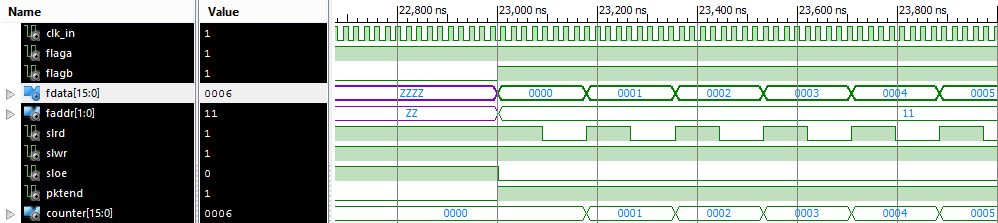
\includegraphics[height=.14\textheight]{sist_tb_lect.png}
		\caption{Simulación del inicio del ciclo de lectura}
		\label{test:tb:lect}
	\end{figure}

	La Figura \ref{test:tb:lect} muestra el diagrama temporal entregado por el simulador en donde se detalla el inicio de la operación de lectura de la memoria de la interfaz USB. Cuando la señal \textit{FLAGB} se encuentra en $'1'$, el sistema activa la memoria FIFO del controlador FX2LP con dirección $''00''$ y habilita también su salida a través de la señal \textit{SLOE}. Luego, procede a leer la memoria colocando en bajo la señal \textit{SLRD}. Una vez leído el dato, el contador generador de datos es incrementado y el nuevo dato es leído con el siguiente flanco descendente de la señal \textit{SLRD}. Esta secuencia es repetida hasta que la señal \textit{FLAGB} sea $'0'$.
	
	\begin{figure}[b]
		\centering
		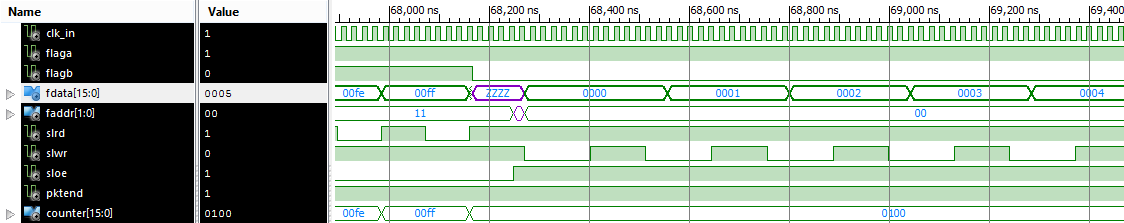
\includegraphics[height=.14\textheight]{sist_tb_esc}
		\caption{Diagrama temporal del final del ciclo de lectura e inicio del ciclo de escritura, entregado por el simulador}
		\label{test:tb:escr}
	\end{figure}

	Cuando fueron leídos todos los datos contenidos en el controlador FX2LP, este colocara en bajo la señal \textit{FLAGB}. Con esta señal,
	el FPGA comenzará el ciclo de escritura, reenviando los datos almacenados en su memoria. En la Figura \ref{test:tb:escr} se puede observar que cuando la señal \textit{FLAGB} baja a $'0'$, se interrumpe el ciclo de lectura y el sistema vuelve al estado de reset, y a continuación, inicia el ciclo de escritura. Durante la operación de escritura, la MEF coloca el bus \textit{FADDR[1:0]} en $''11'$ por el FGPA, activando la memoria FIFO con esta dirección, es decir la receptora de los datos que emite el FPGA. Luego, activa y desactiva, en forma intermitente la señal \textit{SLWR}, enviando los datos almacenados en la memoria del FPGA hacia la memoria de la interfaz.
	
	\begin{figure}[t]
		\centering
		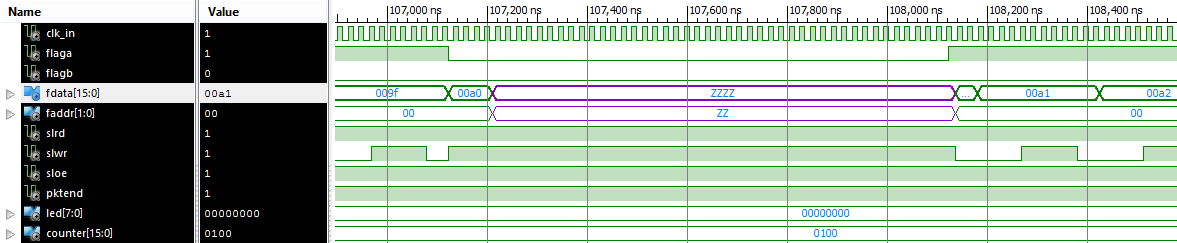
\includegraphics[height=.14\textheight]{sist_tb_esc_int}
		\caption{Simulación de una interrupción en el ciclo de escritura por falta de espacio en la memoria de la interfaz USB}
		\label{test:tb:int}
	\end{figure}
	
	Si por algún motivo la memoria de la interfaz USB se queda sin más espacio para el almacenamiento de los datos que provienen del FPGA, el controlador FX2LP coloca en bajo la señal \textit{FLAGA}. En la Figura \ref{test:tb:int} se observa que luego del flanco negativo de la señal \textit{FLAGA}, el FPGA interrumpe el envío. Cuando la señal \textit{FLAGA} vuelve a $'1'$, la memoria reanuda el envío de los datos almacenados.
	
	\begin{figure}[b]
		\centering
		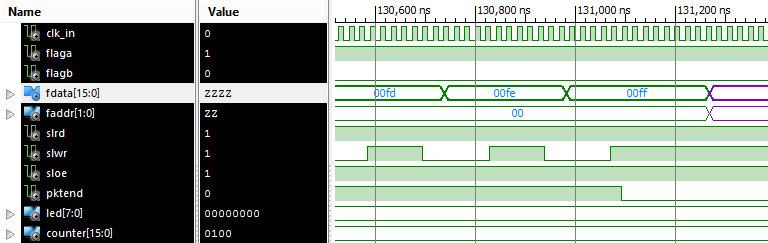
\includegraphics[height=.14\textheight]{sist_tb_pktend.png}
		\caption{Final de la simulación}
		\label{test:tb:pktend}
	\end{figure}

	Una vez que la memoria interna del FPGA no posee más datos para transmitir, la MEF coloca la señal PKTEND en $'0'$, indicando que terminó el envío de datos. Esto se puede observar en la Figura \ref{test:tb:pktend}. Se puede inferir que todos los datos de la memoria fueron transmitidos debido a que el último dato enviado a través del bus de datos es igual al último valor del contador utilizado como generador de datos de entrada al sistema. 
	
	Luego de realizada la simulación y verificado que el funcionamiento del sistema es el esperado, se está en condiciones de cargar la síntesis del circuito en el FPGA. Al elaborar la síntesis, el entrono de desarrollo ISE otorga un informe en donde consta, entre otras cosas, la cantidad de recursos del FPGA que utilizará la síntesis al ser cargada en el circuito integrado. En el caso de este desarrollo, el informe muestra que se utiliza menos del 2\% de los recursos programables del FPGA Spartan 6. Tal vez el punto menos favorable del desarrollo es la cantidad de puertos utilizados, sin embargo quedan disponibles más de 60, lo cual no es un número despreciable . La transcripción del informe se puede observar en el Apéndice~\ref{ap:vhdl}. 
		
\subsection{Carga del sistema de pruebas en el FPGA}
	Para efectuar la carga del sistema fue necesario especificar en el entorno de desarrollo ISE provisto por la compañía Xilinx Inc, en qué pines del FPGA debe asignar cada uno de los puertos descriptos en el código del sistema. Con este propósito, se elabora un archivo denominado \textit{User Constraints File} (que significa Archivo de Restricciones del Usuario) y lleva como extensión la sigla \textit{ucf}. El texto completo de este archivo se observa en el Apéndice \ref{ap:vhdl}.
	
	El archivo \textit{ufc} se generó a través de una interfaz gráfica provista por Xilinx Inc., denominada \textit{Plan Ahead}. En ella se puede cargar en una planilla la equivalencia entre los pines y los puertos, como así también los niveles de tensión lógicos necesarios. En dicha planilla se cargaron los puertos como se indican en la Tabla \ref{tab:fpga:conexion}. Estos puertos fueron configurados utilizando el estándar LVTTL, que es utilizado tanto en la placa Mojo v3~\cite{Mojo}, como en el controlador FX2LP~\cite{Cypress2017}.
	
	Otra configuración indicada en el archivo \textit{ucf} fue la frecuencia de la entrada de reloj. Esta indicación es importante para detectar posibles errores temporales durante la fase de ruteo del compilador. Finalmente, se ejecutó el compilador para elaborar el archivo de configuración del FPGA, el cual fue cargado en la memoria Flash de la placa de desarrollo Mojo v3 y se constató que no existieron errores en la carga.
	